\documentclass[a4paper, 12pt]{article}
\usepackage{changepage, titlesec, hyperref, fullpage}
\usepackage{graphicx}
\titleformat{\section}[block]{\bfseries}{\thesection.}{1em}{}
\titleformat{\subsection}[block]{}{\thesubsection}{1em}{}
\titlespacing*{\subsection} {2em}{3.25ex plus 1ex minus .2ex}{1.5ex plus .2ex}
\title{Architecture Document}
\author{Kara King, Nathaniel Blake, Eric Weyant, Aam Wechter and Erich Harkema}
\begin{document}
\maketitle

\section{Introduction} \label{sec:intro}
\begin{adjustwidth}{2em}{0pt}
\textit{TweetTrunk} is set up in a way so each module has one responsibility. The modules are below with a description of each and the classes that are within them. 
\end{adjustwidth}

\tableofcontents

\section{System Architecture} \label{sec:sysarch}
\begin{adjustwidth}{2em}{0pt}

\begin{figure}[ht!]
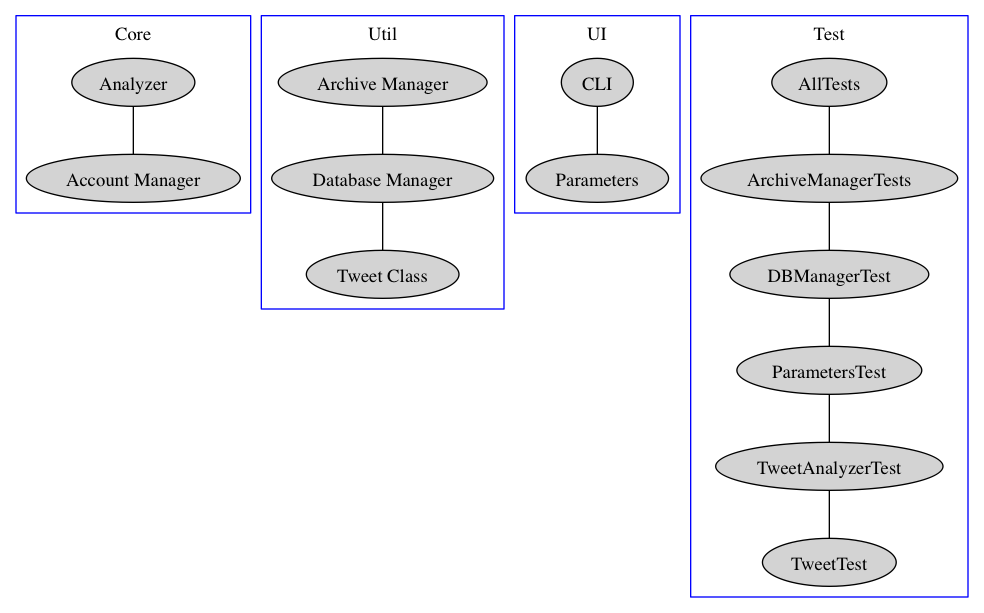
\includegraphics[scale=.5]{architecture.png}
\caption{System Architecture}
\label{Examples}
\end{figure}


\subsection{core} \label{sec:archd}
\begin{adjustwidth}{2em}{0pt}
The core module is used to package together all of the classes that deal with the actual analysis of tweet and authentication of the user to twitter. The classes in this module are \textit{AccountManager.java} and \textit{TweetsAnalyzer.java}. 

\end{adjustwidth}


\subsection{test} \label{sec:archa}
\begin{adjustwidth}{2em}{0pt}
The test module is used to package together all of the test classes for TweetTrunk. This module essentially uses every other module in order to test all of the methods within each class. The classes in this module are \textit{AllTest.java}, \textit{ArchiveManagerTests.java}, \textit{DBManagerTests.java}, \textit{ParametersTest.java}, \textit{TweetsAnalyzerTests.java}, \textit{TweetTests.java}, and \textit{TweetTrunkCLITests.java}.

\end{adjustwidth}


\subsection{ui} \label{sec:archb}
\begin{adjustwidth}{2em}{0pt}
The ui module is used to package together all of the classes that deal with user interactions with TweetTrunk such as classes that deal with command line arguments and parsing JSON files. This module also deals with the use of JCommander that parses the users command line arguments. The classes in this module are \textit{Parameters.java} and \textit{TweetTrunkCLI.java}.


\end{adjustwidth}
\subsection{util} \label{sec:archc}
\begin{adjustwidth}{2em}{0pt}
The util module is used to package together all of the classes that deal with the back end work of TweetTrunk such as database interactions. In addition to that, this module has the tweet class in it which is used in every class within our system to create a tweet object. The classes within this module are \textit{ArchiveManager.java},  \textit{DBManager.java}, and \textit{Tweet.java}. 


\end{adjustwidth}
\end{adjustwidth}



\subsection{Architecture Rationale} \label{sec:rationale}
\begin{adjustwidth}{2em}{0pt}
We wanted to have one point of input and one point of output for our system so we justed TweetTrunkCLI as our driver class for the whole system. This class is the one that the user interacts with directly through their command-line arguments. Then we figured having multiple modules would be a good idea so we would have database creation separate from authentication of the user which would then also be separate from the user interaction with our system. Tests are separate from every other module because they do not deal with the user interaction specifically. The test classes however, rely on every other class. \newline\newline
Besides the classes, we used SQL as our database engine with the use of SQLite. 
\end{adjustwidth}

\end{document}

